%!TEX root=../draft.tex
\section{Experimental Evaluation}
\label{ch5_experiments}

We compare the performance of our linear TM overlays using a set of compute kernels from~\cite{jain2015efficient,binipolynomial}, as shown in Table~\ref{benchmarks}.
The V1 (1 DSP, no WB), V2 (2 DSP, no WB), V3 (WB, IWP=5) and V4 (WB, IWP=4) overlays are compared to the overlay in~\cite{li2016area}. 
V1, V2 and the overlay in~\cite{li2016area} have a depth equal to the critical path, and are configured on a kernel by kernel basis, while V3 and V4 have a fixed depth of eight. 
All overlays are implemented on a Zynq XC7Z020.

The FPGA DSP and logic slice utilization, and operating frequency, for different depth V1 and V2 overlays are shown in Fig.~\ref{scalability} (V3 and V4 are not included in this figure as they have a fixed depth). A depth 8 V1 overlay consumes 654 logic slices and 8 DSP slices which represents less than 5\% of the logic and DSP resources on Zynq. The depth 8 V2 overlay consumes 893 logic slices and 16 DSP blocks or less than 8\% of the Zynq resources. 
By comparison, the fixed depth (of 8) V3 (and V4) overlay consumes 814 (817) logic slices, 8 (8) DSP slices and operates at a frequency of 286MHz (233MHz).

The DFG characteristics (number of I/O, number of arithmetic operations and graph depth) for the chosen benchmarks and the II achieved when mapped to the various overlays are shown in Table~\ref{benchmarks}. For the first three benchmarks, which have a depth $\leq$ 8, ASAP scheduling is used to map to the V3 and V4 overlays, and thus, the II is the same as for the V1 overlay. 
The V1 (V2) overlay has an average 42\% (71\%) reduction in the II, compared to~\cite{li2016area}.
The V3 (V4) overlay has an average 34\% (40\%) reduction in the II for the depth $>$ 8 benchmarks.
%with depth $>$ 8, compared to~\cite{li2016area}.

\begin{comment}
Among the feed-forward only overlays such as~\cite{li2016area}, V1, and V2, their requirement for the number of FUs is determined by the graph depth of each benchmark. 
The II is high for benchmarks with a large number of I/O nodes and high parallelism, where parallelism stands for the average number of operations per schedule stage.
It can be used to roughly measure the throughput, as all the three overlays run at a frequency with a slight degradation from around 330MHz to 300MHz on Zynq XC7Z020, as shown in Fig.~\ref{fmax}. 
According to Table~\ref{benchmarks} and Fig.~\ref{resources}, V1 generally reduces the II into half with almost the same resource consumption as~\cite{li2016area}, and V2 further achieves down to a quarter with an incremental area overhead.
As there are no loop carried dependencies, we can replicate multiple streaming models as in Fig.~\ref{pipelines} to reduce the II into a theoretical minimum of 1.
\end{comment}

\begin{table}[t]
	\renewcommand{\arraystretch}{1}
	\caption{DFG characteristics of benchmark set.}
	\label{benchmarks}
	\centering
%	\scriptsize 
	\small
	\resizebox{\columnwidth}{!}{
		\begin{tabular}{lrrrrrrrr}
			\toprule
			Benchmark & I/O & \#Ops & Depth & II$_{\cite{li2016area}}$ & II$_{V1}$ & II$_{V2}$ & II$_{V3}$ & II$_{V4}$ \\ \midrule
			chebyshev & 1/1 &     7 &     7 &                        6 &         4 &         2 &         4 &         4 \\
			mibench   & 3/1 &    13 &     6 &                       14 &         8 &         4 &         8 &         8 \\
			qspline   & 7/1 &    25 &     8 &                       19 &        11 &       5.5 &        11 &        11 \\
			sgfilter  & 2/1 &    18 &     9 &                       13 &         8 &         4 &         8 &         8 \\
			poly5     & 3/1 &    27 &     9 &                       19 &        11 &       5.5 &        11 &        11 \\
			poly6     & 3/1 &    44 &    11 &                       25 &        14 &         7 &        13 &        12 \\
			poly7     & 3/1 &    39 &    13 &                       24 &        14 &         7 &        20 &        17 \\
			poly8     & 3/1 &    32 &    11 &                       21 &        12 &         6 &        16 &        14 \\ \bottomrule
		\end{tabular}
	}
	
\end{table}

%\pgfdeclarelayer{background}
%\pgfdeclarelayer{foreground}
%\pgfsetlayers{background,main,foreground}

\pgfplotsset{
	axis background/.style={fill=none},
	%tick style=mygrey2,
	%tick label style=mygrey2,
	grid=none,
	%xtick pos=left,
	%ytick pos=left,
	tick style={
		major grid style={style=white,line width=1pt},minor grid style=white,
%		major grid style={style=white,line width=1pt},minor grid style=mygrey3,
		%tick align=outside,
	},
	%minor tick num=4,
}

\begin{figure}[b]
	\centering
	\begin{subfigure}[]{0.23\textwidth}
		\centering	
		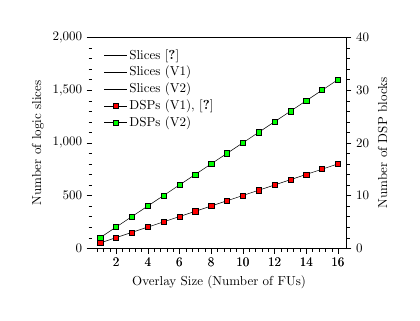
\begin{tikzpicture}[scale = 0.47]
		\begin{axis}[
%		xlabel=Overlay Size (Number of FUs),
		ylabel=Number of logic slices,
		ymax = 2000,
		%ymax = 2500,
		ymin = 0,
		xmax = 16.5,
	    xmin = 0.5,
		legend pos=north west,
		legend cell align={left},
		legend style={draw=none}
		]    
		
		\addplot [mark=*,mark options={fill=blue}] plot coordinates {
			(1,     121)
			(2,     183)
			(3,     274)
			(4,     349)
			(5,     446)
			(6,     505)
			(7,     599)
			(8,     648)
			(9,     692)
			(10,    800)
			(11,    820)
			(12,    925)
			(13,    975)
			(14,    1034)
			(15,    1187)
			(16,    1293)									
		};
		\label{S_olaf}
		\addlegendentry{Slices~\cite{li2016area}}
		
		\addplot [mark=*,mark options={fill=red}] plot coordinates {
			(1,     121)
			(2,     179)
			(3,     272)
			(4,     339)
			(5,     477)
			(6,     530)
			(7,     552)
			(8,     654)
			(9,     775)
			(10,    787)
			(11,    888)
			(12,    969)
			(13,    1028)
			(14,    1165)
			(15,    1235)
			(16,    1292)									
		};
		\label{S_V1}
		\addlegendentry{Slices (V1)}
	
		\addplot [mark=*,mark options={fill=green}] plot coordinates {
			(1,     170)
			(2,     295)
			(3,     374)
			(4,     507)
			(5,     562)
			(6,     671)
			(7,     790)
			(8,     893)
			(9,     1019)
			(10,    1143)
			(11,    1247)
			(12,    1334)
			(13,    1416)
			(14,    1531)
			(15,    1591)
			(16,    1892)			
		};
		\label{S_V2}
		\addlegendentry{Slices (V2)} 
%		\legend{Slices~\cite{li2016area}\\Slices (V1)\\Slices (V2)\\}     
		\end{axis}
		
		\begin{axis}[
		axis y line*=right,
		xlabel=Overlay Size (Number of FUs),
		ylabel=Number of DSP blocks,
		ymax = 40,
		%ymax = 50,
		ymin = 0,
		xmax = 16.5,
	    xmin = 0.5,
		legend pos=north west,
		legend cell align={left},
		legend style={draw=none}
		]
		\addlegendimage{/pgfplots/refstyle=S_olaf}\addlegendentry{Slices~\cite{li2016area}}
		\addlegendimage{/pgfplots/refstyle=S_V1}\addlegendentry{Slices (V1)}
		\addlegendimage{/pgfplots/refstyle=S_V2}\addlegendentry{Slices (V2)}

		\addplot [mark=square*,mark options={fill=red}] plot coordinates {
			(1,     1)
			(2,     2)
			(3,     3)
			(4,     4)
			(5,     5)
			(6,     6)
			(7,     7)
			(8,     8)
			(9,     9)
			(10,    10)
			(11,    11)
			(12,    12)
			(13,    13)
			(14,    14)
			(15,    15)
			(16,    16)		
		};
		\addlegendentry{DSPs (V1),~\cite{li2016area}} 
		
		\addplot [mark=square*,mark options={fill=green}] plot coordinates {
			(1,     2)
			(2,     4)
			(3,     6)
			(4,     8)
			(5,     10)
			(6,     12)
			(7,     14)
			(8,     16)
			(9,     18)
			(10,    20)
			(11,    22)
			(12,    24)
			(13,    26)
			(14,    28)
			(15,    30)
			(16,    32)				
		};
		\addlegendentry{DSPs (V2)}
				
%		\legend{DSPs (V1),~\cite{li2016area}\\DSPs (V2)\\}	
		\end{axis}
		\end{tikzpicture}		
		\caption{Resource Usage}
		\label{resources}
		
	\end{subfigure}
	~
%	\hfill
%	\\
	\begin{subfigure}[]{0.23\textwidth}
		\centering	
	 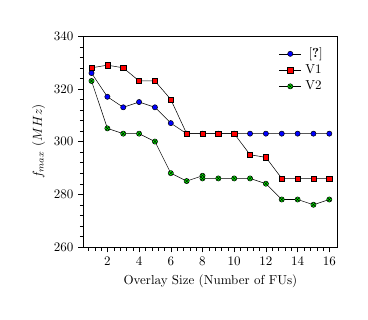
\begin{tikzpicture}[scale = 0.47]
	 \begin{axis}[
	 xlabel=Overlay Size (Number of FUs),
	 ymin=260,
	 ymax=340,
	 %ymin=200,
	 %ymax=400,
	 xmax = 16.5,
	 xmin = 0.5,
	 ylabel=$f_{max}$ ($MHz$),
	 legend pos=north east,
	 legend style={draw=none}
	 ]    

	\addplot [mark=*,mark options={fill=blue}] plot coordinates {
		(1,     326)
		(2,     317)
		(3,     313)
		(4,     315)
		(5,     313)
		(6,     307)
		(7,     303)
		(8,     303)
		(9,     303)
		(10,    303)
		(11,    303)
		(12,    303)
		(13,    303)
		(14,    303)
		(15,    303)
		(16,    303)	
	}; 
	 \addplot [mark=square*,mark options={fill=red}] plot coordinates {
	 	(1,     328)
	 	(2,     329)
	 	(3,     328)
	 	(4,     323)
	 	(5,     323)
	 	(6,     316)
	 	(7,     303)
	 	(8,     303)
	 	(8,     303)
	 	(9,     303)
	 	(10,    303)
	 	(11,    295)
	 	(12,    294)
	 	(13,    286)
	 	(14,    286)
	 	(15,    286)
	 	(16,    286)
	 }; 
	 \addplot [mark=otimes*,mark options={fill=green}] plot coordinates {
	 	(1,     323)
	 	(2,     305)
	 	(3,     303)
	 	(4,     303)
	 	(5,     300)
	 	(6,     288)
	 	(7,     285)
	 	(8,     287)
	 	(8,     286)
	 	(9,     286)
	 	(10,    286)
	 	(11,    286)
	 	(12,    284)
	 	(13,    278)
	 	(14,    278)
	 	(15,    276)
	 	(16,    278) 	
	 };

	 \legend{~\cite{li2016area}\\V1\\V2\\}
	 \end{axis}

	 \end{tikzpicture}	
	 \caption{$f_{max}$ Drop}
	 \label{fmax}
	%}
	\end{subfigure}
	
	\caption[]{V1 and V2 overlay scalability on Zynq XC7Z020.} 
	\label{scalability}
	
\end{figure}



Fig.~\ref{throughput_latency} shows the throughput and latency of the different overlays for the benchmarks given in Table~\ref{benchmarks}. 
In terms of throughput, all overlays have a higher throughput than the overlay of~\cite{li2016area}. This is because interleaving data transfer with execution reduces the II and hence improves throughput.
The two DSP V2 overlay has approximately twice the throughput as the V1 overlay, but also requires twice the data bandwidth. The size of both of these overlays is dependant on the depth (critical path) of the application kernel's DFG, and needs to be reconfigured when the application kernel changes.
A depth 8 V1 (V2) overlay requires a minimum reconfigurable region of 7 (9) CLB tiles and 1 (2) DSP tile with a configuration time of 0.73 (1.02) ms using the processor configuration access port (PCAP). Additionally, the overlays require a further 0.29$\mu s$ to load the configuration data for the largest benchmark.

The single DSP V3 overlay has a throughput similar to the V1 overlay, with an average reduction of just 10\%. The V4 overlay has a slightly reduced throughput as it operates at a lower frequency due to the removal of pipeline registers to reduce the IWP.
The V3 and V4 overlays both have a fixed depth (in these experiments a depth of 8 is used).
Adding write-back capabilities allows larger kernels to be mapped to a smaller number of FUs, removing the requirement that the overlay depth must be the same as the kernel critical path. This eliminates the need to reconfigure the overlay when the application kernel changes, making the overlay more general purpose (but requiring a different scheduling strategy).
Thus, a hardware context switch on the V3 overlay requires just 0.25$\mu s$ for the largest benchmark, representing a 2900$\times$ reduction compared to the V1 overlay.

The latency is heavily dependent on the depth of the overlay. For the V1 and V2 overlays and the overlay of~\cite{li2016area}, the overlay depth is equal to the DFG depth, due to the ASAP scheduling strategy used, and hence these overlays all have a larger latency. The V3 and V4 overlays generally show a significant reduction in the latency, particularly for larger depth DFGs, due to the fixed overlay depth. 



\pgfplotsset{
	axis background/.style={fill=white},
	tick style=black,
	tick label style=black,
	grid=both,
	xtick pos=left,
	ytick pos=left,
	tick style={
		major grid style={style=white,line width=1pt},minor grid style=white,
		tick align=outside,
	},
	minor tick num=4,
}

\begin{figure}[tb]
	\centering
	\begin{subfigure}[]{0.5\textwidth}
		\centering
		\pgfplotstableread{
			0		0.35	0.53	1.00	0.50	0.43
			1		0.29	0.50	0.94	0.46	0.38 
			2		0.40	0.69	1.30	0.65	0.53
			3		0.42	0.68	1.29	0.64	0.52
			4		0.43	0.74	1.40	0.70	0.57
			5		0.53	0.93	1.80	0.97	0.85
			6		0.49	0.80	1.55	0.56	0.53 
			7		0.46	0.79	1.53	0.57	0.53
		}\datathroughput
		\begin{tikzpicture}
		\centering
		\begin{axis}[ybar=0pt,
		width=17cm,
		x = 0.85cm,
		height=4.3cm,
		ymin=0,
		ymax=2,        
		ylabel={Throughput (GOPS)},
		grid style={dotted,gray},
		ymajorgrids=true,
		%	nodes near coords,    
		xtick=data,
		bar width = 0.15,
		xticklabels = {
			\strut 1,
			\strut 2,
			\strut 3,
			\strut 4,
			\strut 5,
			\strut 6,
			\strut 7,
			\strut 8                                   
		},
		x tick label style={rotate=45, anchor=north east, inner sep=0mm},
		major x tick style = {opacity=0},
		minor x tick num = 1,
		minor tick length=1ex,
		%	every node near coord/.append style={
		%		anchor=west,
		%		rotate=90,
		%		font=\tiny
		%	},
		]
		
		\addplot[draw=black,fill=blue, draw opacity=1] table[x index=0,y index=1] \datathroughput;\label{T_olaf}
		\addplot[draw=black,fill=red, draw opacity=1] table[x index=0,y index=2]   \datathroughput;\label{T_V1} 
		\addplot[draw=black,fill=green, draw opacity=1] table[x index=0,y index=3] \datathroughput;\label{T_V2} 
		\addplot[draw=black,fill=yellow, draw opacity=1] table[x index=0,y index=4] \datathroughput;\label{T_V3} 
		\addplot[draw=black,fill=cyan, draw opacity=1] table[x index=0,y index=5]  \datathroughput;\label{T_V4} 
		
		\end{axis}
		\node [draw=none, fill=white] at (rel axis cs: 0.55,1.2) {\shortstack[l]{
				\ref{T_olaf}~\cite{li2016area} \ref{T_V1} V1 \ref{T_V2} V2} \ref{T_V3} V3 \ref{T_V4} V4};	
		\end{tikzpicture}
%		\caption{Throughput in GOPS.}
		\label{throughput}
	\end{subfigure}
	
	\begin{subfigure}[]{0.5\textwidth}
		\centering
		\pgfplotstableread{
			0		116	116	123	105	129
			1		143	139	154	105	129
			2		235	235	249	147	181
			3		198	198	210	151	181
			4		248	248	263	165	198
			5		373	385	396	200	224
			6		400	424	436	231	258
			7		320	330	340	203	237
		}\datalatency
		\begin{tikzpicture}
		\centering
		\begin{axis}[ybar=0pt,
		width=17cm,
		x = 0.85cm,
		height=4.3cm,
		ymin=0,
		ymax=500,        
		ylabel={Latency (ns)},
		grid style={dotted,gray},
		ymajorgrids=true,
		%	nodes near coords,    
		xtick=data,
		bar width = 0.15,
		xticklabels = {
			\strut 1,
			\strut 2,
			\strut 3,
			\strut 4,
			\strut 5,
			\strut 6,
			\strut 7,
			\strut 8                                   
		},
		x tick label style={rotate=45, anchor=north east, inner sep=0mm},
		major x tick style = {opacity=0},
		minor x tick num = 1,
		minor tick length=1ex,
		%	every node near coord/.append style={
		%		anchor=west,
		%		rotate=90,
		%		font=\tiny
		%	},
		]
		
		\addplot[draw=black,fill=blue, draw opacity=1] table[x index=0,y index=1] \datalatency;\label{L_olaf}
		\addplot[draw=black,fill=red, draw opacity=1] table[x index=0,y index=2] \datalatency;\label{L_V1} 
		\addplot[draw=black,fill=green, draw opacity=1] table[x index=0,y index=3] \datalatency;\label{L_V2} 
		\addplot[draw=black,fill=yellow, draw opacity=1] table[x index=0,y index=4] \datalatency;\label{L_V3} 
		\addplot[draw=black,fill=cyan, draw opacity=1] table[x index=0,y index=5] \datalatency;\label{L_V4} 
		
		\end{axis}
%		\node [draw=none, fill=white] at (rel axis cs: 0.5,0.85) {\shortstack[l]{
%				\ref{L_olaf}~\cite{li2016area}  \ref{L_V1} V1  \ref{L_V2} V2} \ref{L_V3} V3 \ref{L_V4} V4};	
		\end{tikzpicture}
%		\caption{Latency in ns.}
		\label{latency}
	\end{subfigure}
	
	\caption{Throughput and latency for the benchmarks.}
	\label{throughput_latency}
\end{figure}

\begin{comment}
To demonstrate the benefits of the proposed linear TM overlays, we compare different versions of the linear TM overlays with one of the more efficient spatially configured overlays from the literature~\cite{jain2015efficient}.
For all the implementations we use the minimal number of FUs/hardware for the benchmark implementations, except for V4 with a fix architecture of 8 FUs.
This is to observe the effect of FU reduction on the area requirement, and the benefit of mapping all the benchmarks without overlay reconfiguration.
Fig.~\ref{fu_comparison} shows the number of FUs required for the linear TM overlay V1/V2 compared to that of the spatially configured overlay in~\cite{jain2015efficient} for each of the benchmarks in Table~\ref{benchmarks}. 
There is a significant reduction in the number of FUs required for V1/V2, but at the expense of an increase in the II compared to~\cite{jain2015efficient}. 
The most remarkable advantage of V4 is that it can handle all the benchmarks regardless of the graph depth, which significantly reduce the context switch time for different compute kernels.

%\pgfplotsset{
	axis background/.style={fill=white},
	tick style=black,
	tick label style=black,
	grid=both,
	xtick pos=left,
	ytick pos=left,
	tick style={
		major grid style={style=white,line width=1pt},minor grid style=white,
		tick align=outside,
	},
	minor tick num=4,
}

\begin{figure}[tb]
%\vspace{-18pt}
\centering
%\pgfplotstableread{
%	0  5			7     
%	1  12      		9     
%	2  8	     	6      
%	3  22    		8 
%	4  17    		9      
%	5  30     		11    
%	6  28     		13       
%	7  19      		11
%}\dataset
\pgfplotstableread{
	0  		 5		7     8
	1  		 12     9     8
	2  		 8	    6     8 
	3  		 22    	8 	  8
	4  	 	 17    	9     8
	5  		 30     11    8
	6  		 28     13    8
	7  		 19     11    8
}\dataset
\begin{tikzpicture}
\centering
\begin{axis}[ybar=0pt,
%enlarge x limits=0.05,
width=17cm,
x = 0.85cm,
height=4.3cm,
ymin=0,
ymax=100,        
ylabel={Number of FUs required},
grid style={dotted,gray},
ymajorgrids=true,
nodes near coords,    
xtick=data,
bar width = 0.25,
%xticklabels={1,2,...,26},
xticklabels = {
	\strut 1,
	\strut 2,
	\strut 3,
	\strut 4,
	\strut 5,
	\strut 6,
	\strut 7,
	\strut 8
%	\strut 26 (1)                                    
},
x tick label style={rotate=45, anchor=north east, inner sep=0mm},
major x tick style = {opacity=0},
minor x tick num = 1,
minor tick length=1ex,
every node near coord/.append style={
        anchor=west,
        rotate=90,
        font=\tiny
},
]

\addplot[draw=black,fill=blue!80, draw opacity=1] table[x index=0,y index=1] 
\dataset; \label{scoverlay}
\addplot[draw=black,fill=black!70, draw opacity=1] table[x index=0,y index=2] \dataset;\label{tmoverlay_1} 
\addplot[draw=black,fill=green!60, draw opacity=1] table[x index=0,y index=3] \dataset;\label{tmoverlay_2} 

\end{axis}
	\node [draw=none, fill=white] at (rel axis cs: 0.5,0.72) {\shortstack[l]{
			\ref{scoverlay} Spatially Configured Overlay~\cite{jain2015efficient} \\ \ref{tmoverlay_1} V1/V2 \\ \ref{tmoverlay_2} V4}};

\end{tikzpicture}
\caption{Number of FUs required for the benchmarks.}
\label{fu_comparison}
%\vspace{-9pt}
\end{figure}
\end{comment}
